%%%%%%%%%%%%%%%%%%%%%%%%%%%%%%%%%%%%%%%%%%%%%%%%%%%%%%%%%%%%%%%%%%%%%%%%%%%%%%%%%%%%%%%%%%%%%%%%%%%
%%%%%%%%%%%%%%%%%%%%%%%%%%%%%%%%%%%%%%%%%%%%%%%%%%%%%%%%%%%%%%%%%%%%%%%%%%%%%%%%%%%%%%%%%%%%%%%%%%%
\chapter{Resultados}

Como se mencion\'o previamente, este trabajo se ha basado en los registros de PSG de 6 adultos
mayores con deterioro cognitivo (DC) y 3 sin este padecimiento. La calidad de deterioro
cognitivo fue medida a trav\'es de una bater\'ia de pruebas neuropsicol\'ogicas;
adicionalmente, se midi\'o su posible depresi\'on geri\'atrica. 
En e cuadro \ref{sujetos} se resume esta informaci\'on.

\begin{table}
\centering
\begin{tabular}{l|cc}
Sujeto & Deterioro cogn. & Depresi\'on
\\
\hline
MJNN &   &   \\
RLMN & X &   \\
JANA &   & X \\
CLMN & X &   \\
JGMN & X &   \\
RRMN & X &   \\
VCNN &   &   \\
FGH  & X & ? \\
GURM & ? & ? \\
%& & \\
%& & \\
\end{tabular}
\caption{Caracter\'isticas de los adultos mayores considerados en el estudio, en cuanto
a deterioro cognitivo y depresi\'on geri\'atrica. 
%Las dos primeras letras fueron dadas por sus nombre mientras que las \'ultimas dos son
%mnemotecnias de sus caracter\'isticas: \textbf{M}= mean, \textbf{N}=normal, \textbf{A}=anormal.
Para m\'as detalles consultar \cite{VazquezTagle16}}
\label{sujetos}
\end{table}

Estos gr\'aficos muestran una distribuci\'ion temporal y pseudo-espacial 
de las \'epocas que fueron clasificadas como {no-estacionarias} seg\'un el test PSR
(ver secci\'on [?] para m\'as detalles). 
%M\'as que eso, esta distribuci\'on gr\'afica puede extenderse a otros an\'alisis.

Un primer tratamiento cualitativo que se dio a los resultados obtenidos del test PSR es su
disposici\'on gr\'afica
%Una vez se hubo realizado el test para todas las \'epocas consideradas, se dispuso de los 
%resultados de manera gr\'afica  
como se muestra en las figuras \ref{ejemplo1}.
Por cada canal de PSG (EEG, EOG y EMG), se colocaron en l\'inea horizontal un cuadro por cada
\'epoca en blanco o negro seg\'un el segmento referido haya sido clasificado como
no-estacionario o posiblemente estacionario; posteriormente se han colocado verticalmente las
l\'ineas as\'i obtenidas de todos los canales.
Esta disposici\'on gr\'afica pretende ser consistente con las representaciones gr\'aficas
usuales de EEG, tomando en cuanta una escala m\'as amplia de tiempo gracias a que por
cada \'epoca s\'olo se ha obtenido un dato.
Los gr\'aficos as\'i obtenidos se incluyen como anexo.

\begin{figure}
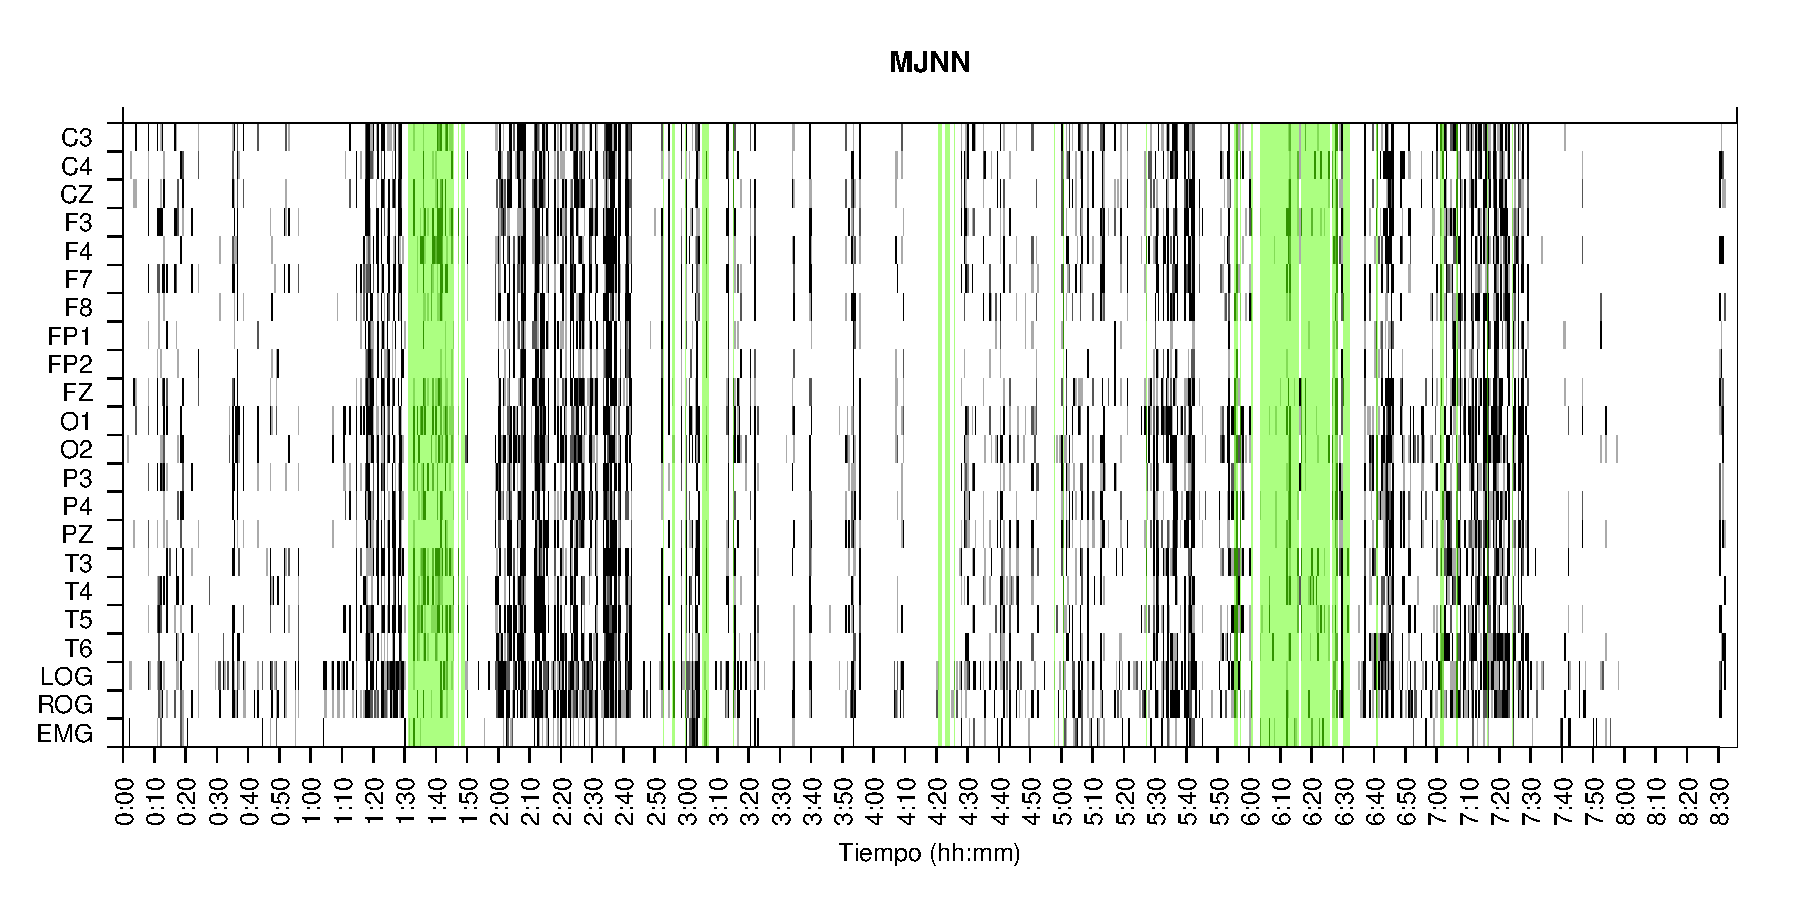
\includegraphics[width=\textwidth]{MJNNVIGILOS_127_mor127_tot1032_esttotal.pdf} 
\caption{Disposici\'on gr\'afica para los resultados del test PSR en el sujeto MJH, 
para 1032 \'epocas de sue\~no y 22 canales. 
En el eje horizontal se muestra el tiempo desde el inicio de registro, en el eje vertical se muestra al 
nombre del canal. 
Se han resaltado con color verde las \'epocas clasificadas como sue\~no MOR (ver texto), que son 127.
Para este gr\'afico se consider\'o con un p-valor cr\'itico de 0.01 para la hip\'otesis
de estacionariedad. Ver texto para m\'as detalles.}
\label{ejemplo1}
\end{figure}

%\begin{figure}
%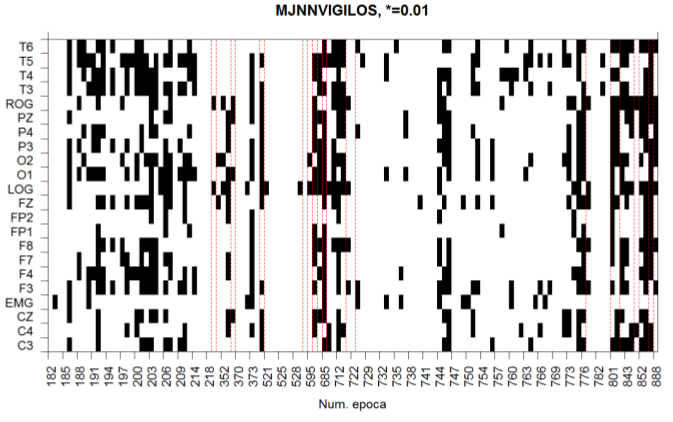
\includegraphics[width=\textwidth]{est02.png} 
%\caption{En este gráfico sólo se ilustran épocas MOR. Las líneas punteadas separan bloques continuos.
%Total de épocas: 1032 , Épocas MOR: 127}
%\label{ejemplo2}
%\end{figure}

La cantidad de \'epocas que no fueron para las cueles no es posible rechazar la hip\'otesis de
estacionariedad ($\alpha=0.05$)
clasificadas como ''\'Epocas Posiblemente Estacionarias'' (EPE).
Como un segundo an\'alisis,
la proporci\'on de EPE con respecto al total de \'epocas registradas fue comparado contra la misma
cantidad restringida \'unicamente a \'epocas correspondientes a sue\~no MOR; la comparaci\'on 
se realiz\'o usando una prueba $\chi^{2}$ de proporciones.
Tanto las proporciones como las diferencias significativas se encuentran en la tabla

\begin{table}
\centering
\begin{tabularx}{\hsize}{c|cc|cc|cc}
Canal&Total&&NMOR&&MOR&\\
&Estacionarios&Porcentaje&Estacionarios&Porcentaje&Estacionarios&Porcentaje\\
\hline
C3&325&31.6\%&285&33.0\%&40&24.1\%\\
C4&339&32.9\%&306&35.4\%&33&19.9\%\\
CZ&318&30.9\%&289&33.4\%&29&17.5\%\\
EMG&96&9.3\%&91&10.5\%&5&3.0\%\\
F3&247&24.0\%&220&25.5\%&27&16.3\%\\
F4&241&23.4\%&233&27.0\%&8&4.8\%\\
F7&220&21.4\%&214&24.8\%&6&3.6\%\\
F8&196&19.0\%&194&22.5\%&2&1.2\%\\
FP1&244&23.7\%&243&28.1\%&1&0.6\%\\
FP2&234&22.7\%&232&26.9\%&2&1.2\%\\
FZ&298&28.9\%&271&31.4\%&27&16.3\%\\
LOG&556&54.0\%&541&62.6\%&15&9.0\%\\
O1&271&26.3\%&239&27.7\%&32&19.3\%\\
O2&279&27.1\%&255&29.5\%&24&14.5\%\\
P3&349&33.9\%&313&36.2\%&36&21.7\%\\
P4&327&31.7\%&301&34.8\%&26&15.7\%\\
PZ&295&28.6\%&278&32.2\%&17&10.2\%\\
ROG&581&56.4\%&553&64.0\%&28&16.9\%\\
T3&221&21.5\%&174&20.1\%&47&28.3\%\\
T4&206&20.0\%&193&22.3\%&13&7.8\%\\
T5&362&35.1\%&304&35.2\%&58&34.9\%\\
T6&323&31.4\%&301&34.8\%&22&13.3\%\\
\end{tabular}
\end{table}

%Me siento particularmente orgulloso
%de haber dise\~nado este tipo de gr\'aficos, ya que  organizan datos que ya se ten\'ian
%y dejan la sensaci\'on de portar nueva informaci\'on.

%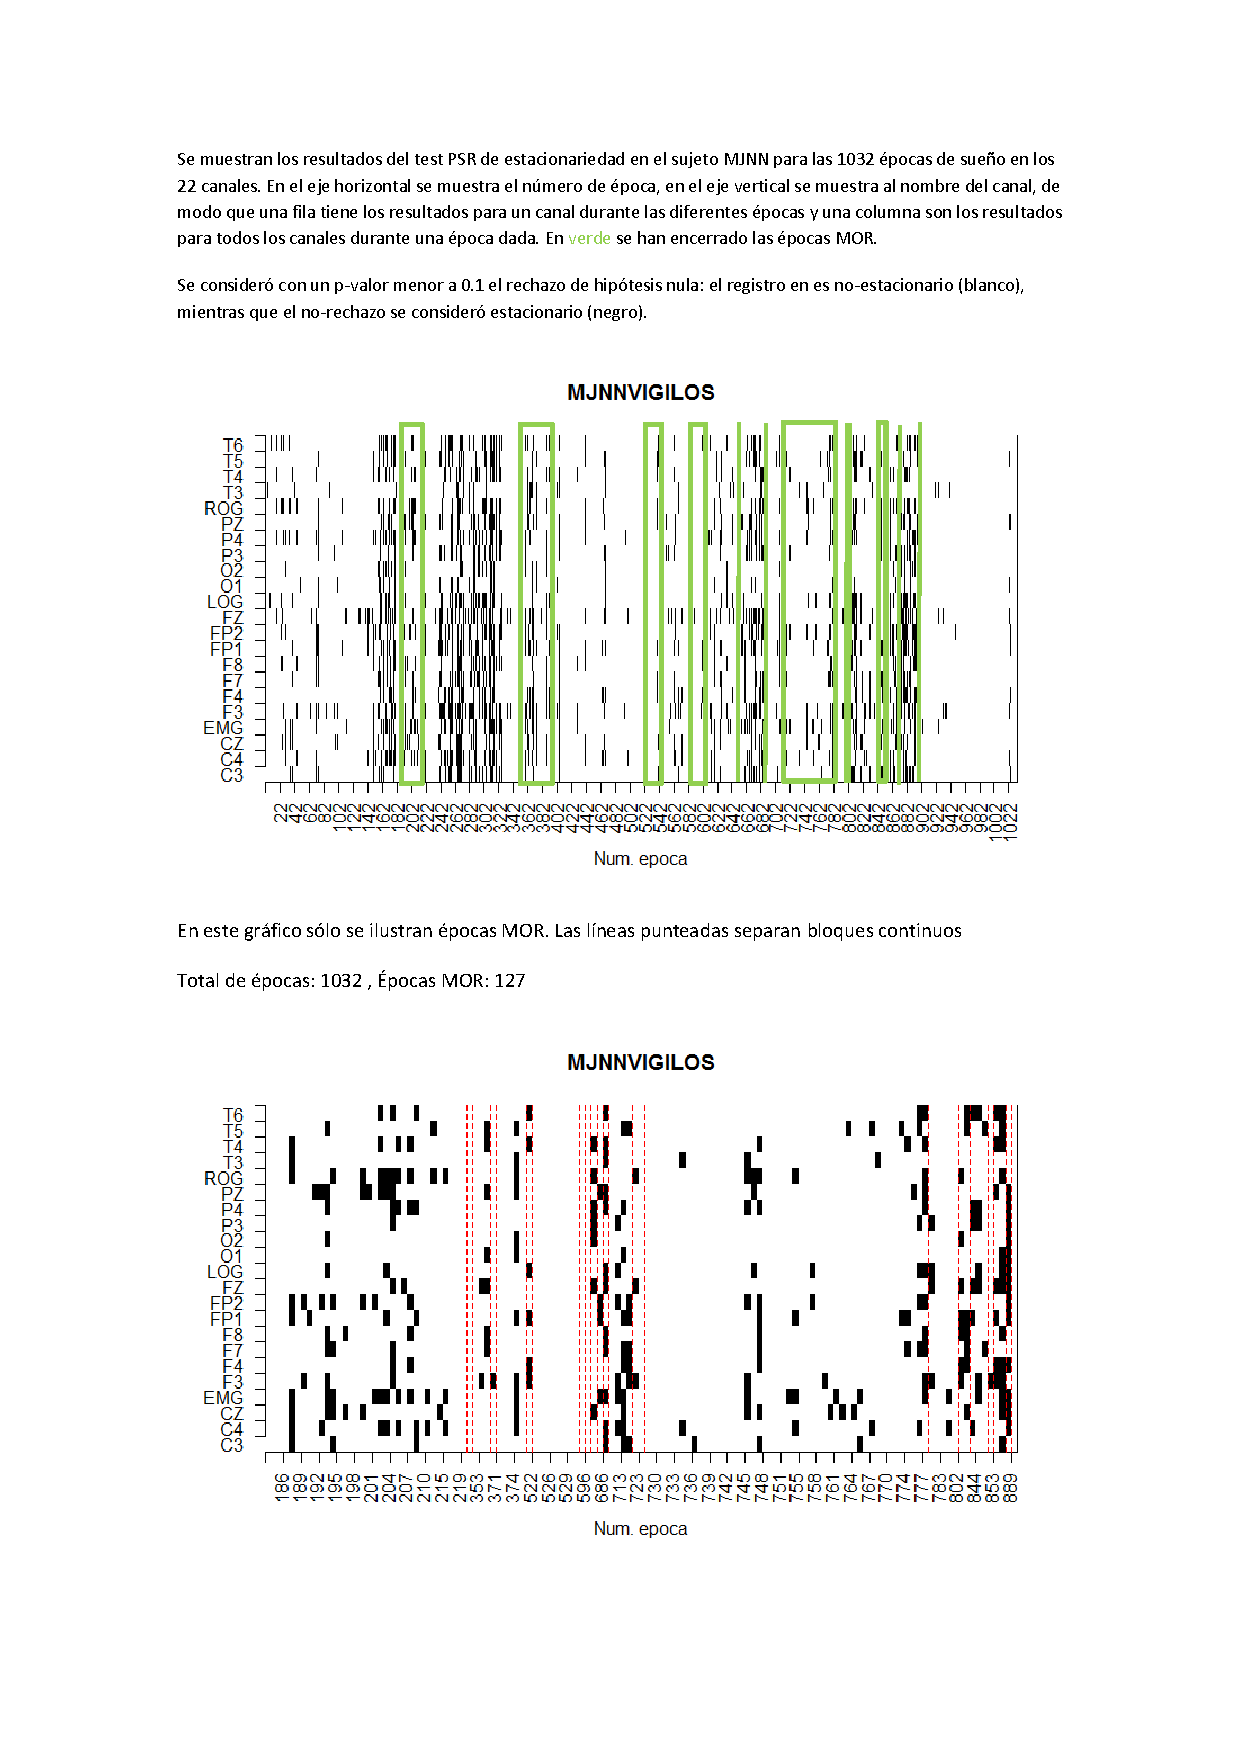
\includepdf[pages={1-},scale=.85]{reporte_de_estacionariedad_170120.pdf}
%
%\afterpage{%
%    \clearpage% Flush earlier floats (otherwise order might not be correct)
%    \thispagestyle{empty}% empty page style (?)
%    \begin{landscape}% Landscape page
%        \centering % Center table
%        \begin{figure}
%            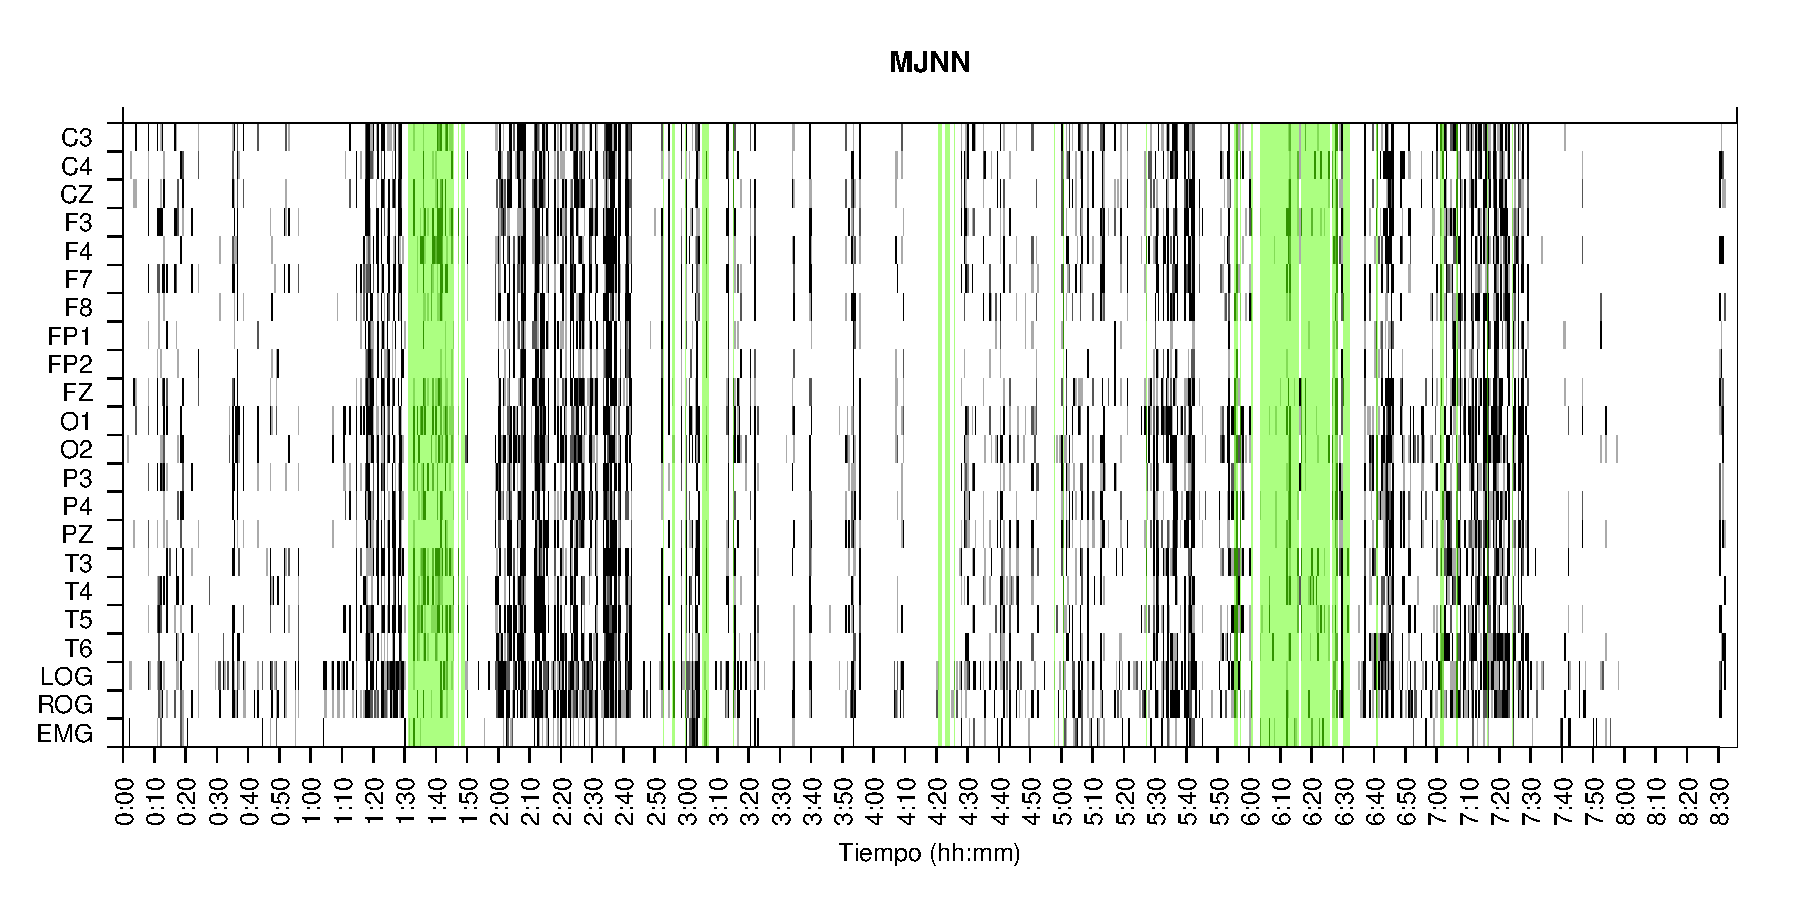
\includegraphics[width=\textwidth]{MJNNVIGILOS_127_mor127_tot1032_esttotal.pdf} 
%            \caption{Total de \'epocas: 1032, \'epocas MOR: 127}
%            %\label{ejemplo1}
%        \end{figure}
%    \end{landscape}
%    \clearpage% Flush page
%}

%%%%%%%%%%%%%%%%%%%%%%%%%%%%%%%%%%%
%%%%%%%%%%%%%%%%%%%%%%%%%%%%%%%%%%%

%\section{Compilados gr\'aficos}
%
%\begin{SidewaysFigure}
%\centering
%\includegraphics[width=\linewidth]
%{./material_bonito170220/MJNNVIGILOS_127_mor127_tot1032_est_total.pdf} 
%\caption{Sujeto: MJNN | Total \'epocas: 1032 | \'Epocas MOR: 127}
%%\label{primera}
%\end{SidewaysFigure}
%\begin{SidewaysFigure}
%\centering
%\includegraphics[width=\linewidth]
%{./material_bonito170220/MJNNVIGILOS_127_mor127_tot127_est_mor.pdf} 
%\caption{Sujeto: MJNN | \'Epocas MOR: 127 | (\'Unicamente \'epocas MOR)}
%%\label{primera}
%\end{SidewaysFigure}
%
%\begin{figure}
%\centering
%\includegraphics[width=\linewidth]
%{./material_bonito170220/porcentaje_bis/MJNNVIGILOS_127_1032_1_bar_porcentaje.pdf} 
%\caption{Sujeto: MJNN | Porcentaje de \'epocas \textit{posiblemente estacionarias}}
%\end{figure}
%
%%%%%%%%%%%%%%%%%%%%%%%%%%%%%%%%%%%%
%%%%%%%%%%%%%%%%%%%%%%%%%%%%%%%%%%%%
%
%\begin{SidewaysFigure}
%\centering
%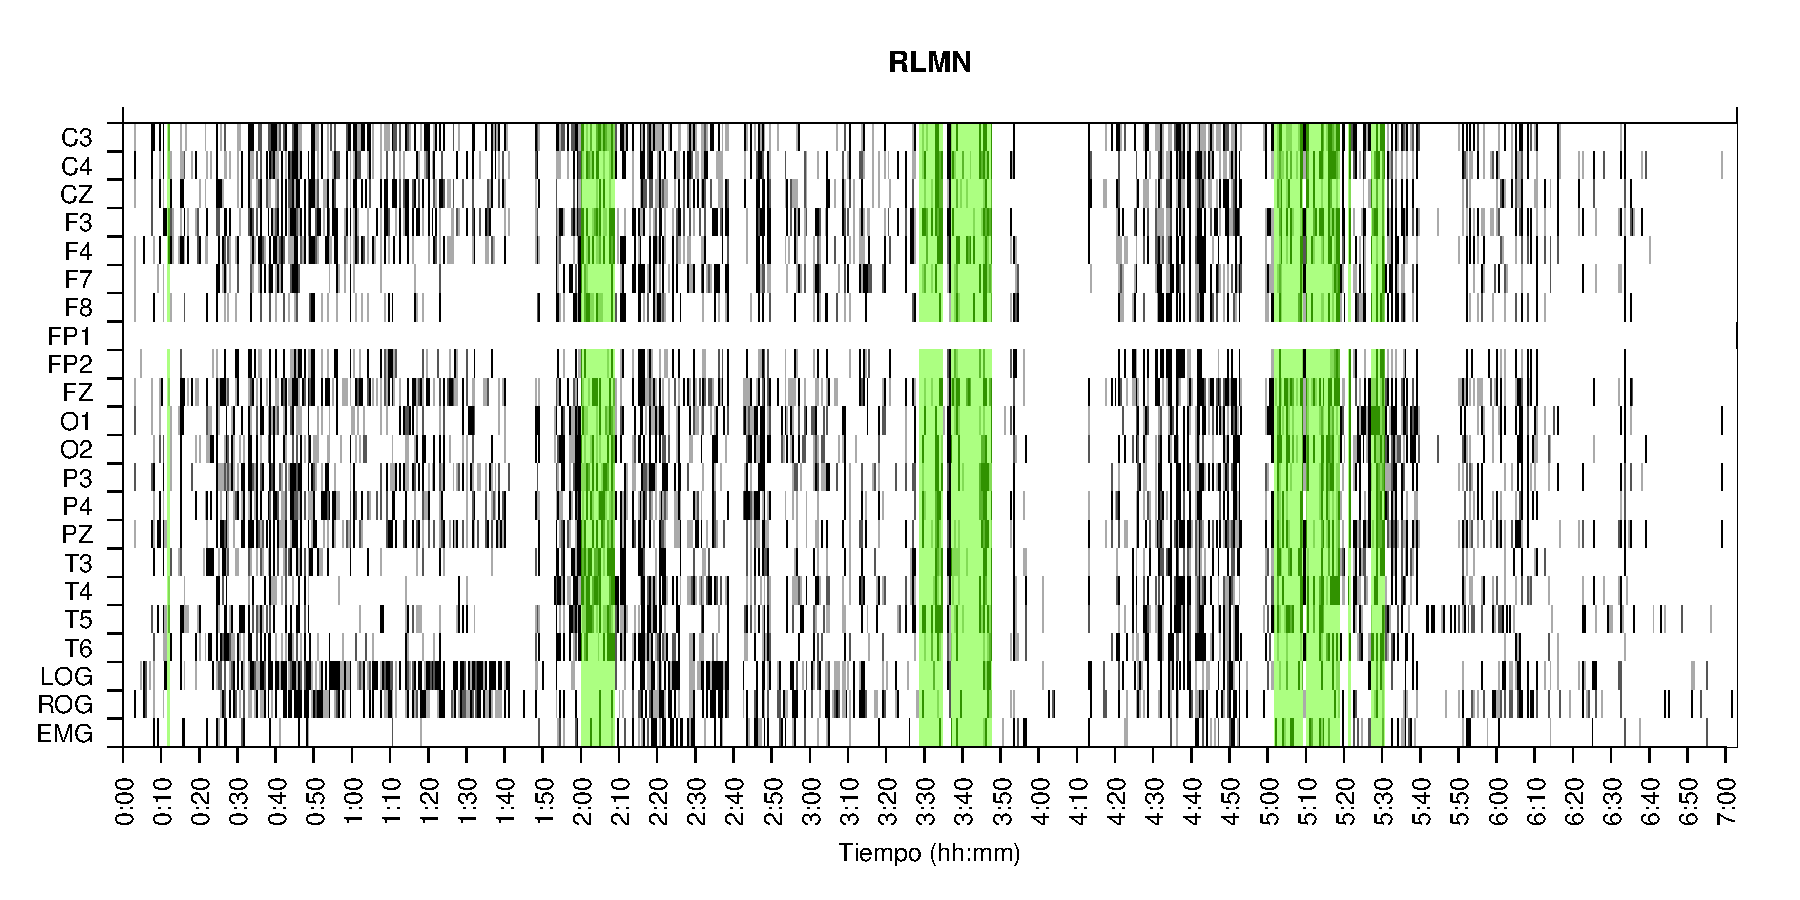
\includegraphics[width=\linewidth]{./material_bonito170220/RLMN10SUE_99_mor99_tot846_est_total.pdf} 
%\caption{Sujeto: RLMN | Total \'epocas: 846 | \'Epocas MOR: 99}
%%\label{primera}
%\end{SidewaysFigure}
%\begin{SidewaysFigure}
%\centering
%\includegraphics[width=\linewidth]
%{./material_bonito170220/RLMN10SUE_99_mor99_tot99_est_mor.pdf} 
%\caption{Sujeto: RLMN | \'Epocas MOR: 99 | (\'Unicamente \'epocas MOR)}
%%\label{primera}
%\end{SidewaysFigure}
%
%\begin{figure}
%\centering
%\includegraphics[width=\linewidth]
%{./material_bonito170220/porcentaje_bis/RLMN10SUE_99_846_1_bar_porcentaje.pdf} 
%\caption{Sujeto: RLMN | Porcentaje de \'epocas \textit{posiblemente estacionarias}}
%\end{figure}
%
%%%%%%%%%%%%%%%%%%%%%%%%%%%%%%%%%%%%
%%%%%%%%%%%%%%%%%%%%%%%%%%%%%%%%%%%%
%
%\begin{SidewaysFigure}
%\centering
%\includegraphics[width=\linewidth]
%{./material_bonito170220/JANASUE_103_mor103_tot907_est_total.pdf} 
%\caption{Sujeto: JANA | Total \'epocas: 907 | \'Epocas MOR: 103}
%%\label{primera}
%\end{SidewaysFigure}
%\begin{SidewaysFigure}
%\centering
%\includegraphics[width=\linewidth]
%{./material_bonito170220/JANASUE_103_mor103_tot103_est_mor.pdf} 
%\caption{Sujeto: JANA | \'Epocas MOR: 103 | (\'Unicamente \'epocas MOR)}
%%\label{primera}
%\end{SidewaysFigure}
%
%\begin{figure}
%\centering
%\includegraphics[width=\linewidth]
%{./material_bonito170220/porcentaje_bis/JANASUE_103_907_1_bar_porcentaje.pdf} 
%\caption{Sujeto: JANA | Porcentaje de \'epocas \textit{posiblemente estacionarias}}
%\end{figure}
%
%%%%%%%%%%%%%%%%%%%%%%%%%%%%%%%%%%%%
%%%%%%%%%%%%%%%%%%%%%%%%%%%%%%%%%%%%
%
%\begin{SidewaysFigure}
%\centering
%\includegraphics[width=\linewidth]
%{./material_bonito170220/CLMN10SUE_132_mor132_tot944_est_total.pdf} 
%\caption{Sujeto: CLMN | Total \'epocas: 944 | \'Epocas MOR: 132}
%%\label{primera}
%\end{SidewaysFigure}
%\begin{SidewaysFigure}
%\centering
%\includegraphics[width=\linewidth]
%{./material_bonito170220/CLMN10SUE_132_mor132_tot132_est_mor.pdf} 
%\caption{Sujeto: CLMN | \'Epocas MOR: 132 | (\'Unicamente \'epocas MOR)}
%%\label{primera}
%\end{SidewaysFigure}
%
%\begin{figure}
%\centering
%\includegraphics[width=\linewidth]
%{./material_bonito170220/porcentaje_bis/CLMN10SUE_132_944_1_bar_porcentaje.pdf} 
%\caption{Sujeto: CLMN | Porcentaje de \'epocas \textit{posiblemente estacionarias}}
%\end{figure}
%
%%%%%%%%%%%%%%%%%%%%%%%%%%%%%%%%%%%%
%%%%%%%%%%%%%%%%%%%%%%%%%%%%%%%%%%%%
%
%\begin{SidewaysFigure}
%\centering
%\includegraphics[width=\linewidth]
%{./material_bonito170220/CLMN10SUE_132_mor132_tot944_est_total.pdf} 
%\caption{Sujeto: JGMN | Total \'epocas: 1207 | \'Epocas MOR: 33}
%%\label{primera}
%\end{SidewaysFigure}
%\begin{SidewaysFigure}
%\centering
%\includegraphics[width=\linewidth]
%{./material_bonito170220/JGMN6SUE_33_mor33_tot33_est_mor.pdf} 
%\caption{Sujeto: CLMN | \'Epocas MOR: 33 | (\'Unicamente \'epocas MOR)}
%%\label{primera}
%\end{SidewaysFigure}
%
%\begin{figure}
%\centering
%\includegraphics[width=\linewidth]
%{./material_bonito170220/porcentaje_bis/JGMN6SUE_33_1207_1_bar_porcentaje.pdf} 
%\caption{Sujeto: JGMN | Porcentaje de \'epocas \textit{posiblemente estacionarias}}
%\end{figure}
%
%%%%%%%%%%%%%%%%%%%%%%%%%%%%%%%%%%%%
%%%%%%%%%%%%%%%%%%%%%%%%%%%%%%%%%%%%
%
%\begin{SidewaysFigure}
%\centering
%\includegraphics[width=\linewidth]
%{./material_bonito170220/RRMNS_114_mor114_tot1244_est_total_bis.pdf} 
%\caption{Sujeto: RRMN | Total \'epocas: 1244 | \'Epocas MOR: 114}
%%\label{primera}
%\end{SidewaysFigure}
%\begin{SidewaysFigure}
%\centering
%\includegraphics[width=\linewidth]
%{./material_bonito170220/RRMNS_114_mor114_tot114_est_mor_bis.pdf} 
%\caption{Sujeto: RRMN | \'Epocas MOR: 114 | (\'Unicamente \'epocas MOR)}
%%\label{primera}
%\end{SidewaysFigure}
%
%\begin{figure}
%\centering
%\includegraphics[width=\linewidth]
%{./material_bonito170220/porcentaje_bis/RRMNS_114_1244_1_bar_porcentaje.pdf} 
%\caption{Sujeto: RRMN | Porcentaje de \'epocas \textit{posiblemente estacionarias}}
%\end{figure}
%
%%%%%%%%%%%%%%%%%%%%%%%%%%%%%%%%%%%%
%%%%%%%%%%%%%%%%%%%%%%%%%%%%%%%%%%%%
%
%\begin{SidewaysFigure}
%\centering
%\includegraphics[width=\linewidth]
%{./material_bonito170220/VCNNS1_200_mor200_tot2584_est_total.pdf} 
%\caption{Sujeto: VCNN | Total \'epocas: 2586 | \'Epocas MOR: 200}
%%\label{primera}
%\end{SidewaysFigure}
%\begin{SidewaysFigure}
%\centering
%\includegraphics[width=\linewidth]
%{./material_bonito170220/VCNNS1_200_mor200_tot200_est_mor.pdf} 
%\caption{Sujeto: VCNN | \'Epocas MOR: 200 | (\'Unicamente \'epocas MOR)}
%%\label{primera}
%\end{SidewaysFigure}
%
%\begin{figure}
%\centering
%\includegraphics[width=\linewidth]
%{./material_bonito170220/porcentaje_bis/VCNNS1_200_2584_1_bar_porcentaje.pdf} 
%\caption{Sujeto: VCNN | Porcentaje de \'epocas \textit{posiblemente estacionarias}}
%\end{figure}
%
%%%%%%%%%%%%%%%%%%%%%%%%%%%%%%%%%%%%
%%%%%%%%%%%%%%%%%%%%%%%%%%%%%%%%%%%%
%
%\begin{SidewaysFigure}
%\centering
%\includegraphics[width=\linewidth]
%{./material_bonito170220/FGHSUE_22_mor22_tot405_est_total.pdf} 
%\caption{Sujeto: FGH | Total \'epocas: 405 | \'Epocas MOR: 22}
%%\label{primera}
%\end{SidewaysFigure}
%\begin{SidewaysFigure}
%\centering
%\includegraphics[width=\linewidth]
%{./material_bonito170220/FGHSUE_22_mor22_tot22_est_mor.pdf} 
%\caption{Sujeto: FGH | \'Epocas MOR: 22 | (\'Unicamente \'epocas MOR)}
%%\label{primera}
%\end{SidewaysFigure}
%
%\begin{figure}
%\centering
%\includegraphics[width=\linewidth]
%{./material_bonito170220/porcentaje_bis/FGHSUE_22_405_1_bar_porcentaje.pdf} 
%\caption{Sujeto: FGH | Porcentaje de \'epocas \textit{posiblemente estacionarias}}
%\end{figure}
%
%%%%%%%%%%%%%%%%%%%%%%%%%%%%%%%%%%%%
%%%%%%%%%%%%%%%%%%%%%%%%%%%%%%%%%%%%
%
%\begin{SidewaysFigure}
%\centering
%\includegraphics[width=\linewidth]
%{./material_bonito170220/GH24031950SUENO_267_mor267_tot3281_est_total.pdf} 
%\caption{Sujeto: GURM | Total \'epocas: 3281 | \'Epocas MOR: 267}
%%\label{primera}
%\end{SidewaysFigure}
%\begin{SidewaysFigure}
%\centering
%\includegraphics[width=\linewidth]
%{./material_bonito170220/GH24031950SUENO_267_mor267_tot267_est_mor.pdf} 
%\caption{Sujeto: GURM | \'Epocas MOR: 267 | (\'Unicamente \'epocas MOR)}
%%\label{primera}
%\end{SidewaysFigure}
%
%\begin{figure}
%\centering
%\includegraphics[width=\linewidth]
%{./material_bonito170220/porcentaje_bis/GH24031950SUENO_267_3281_1_bar_porcentaje.pdf} 
%\caption{Sujeto: GURM | Porcentaje de \'epocas \textit{posiblemente estacionarias}}
%\end{figure}

%%%%%%%%%%%%%%%%%%%%%%%%%%%%%%%%%%%
%%%%%%%%%%%%%%%%%%%%%%%%%%%%%%%%%%%

%%%%%%%%%%%%%%%%%%%%%%%%%%%%%%%%%%%%%%%%%%%%%%%%%%%%%%%%%%%%%%%%%%%%%%%%%%%%%%%%%%%%%%%%%%%%%%%%%%%
%%%%%%%%%%%%%%%%%%%%%%%%%%%%%%%%%%%%%%%%%%%%%%%%%%%%%%%%%%%%%%%%%%%%%%%%%%%%%%%%%%%%%%%%%%%%%%%%%%%